\documentclass[11pt, a4paper, spanish]{article}

\usepackage[a4paper, margin=2.5cm, top=3.5cm, bottom=3.5cm]{geometry} % Define los márgenes
\usepackage{amsmath, amscd, amssymb, amsthm, latexsym} % Paquetes matemáticos
\usepackage[spanish]{babel} % Traduce los paquetes a español
\usepackage[utf8]{inputenc} % Codificación UTF8
\usepackage{fancyhdr} % Encabezados y pies de página
  \pagestyle{fancyplain}
\usepackage{enumerate}
\usepackage{xspace}
\usepackage[page, toc]{appendix} % Apéndices
\usepackage[nottoc, numbib]{tocbibind} % Referencias en la TDC
\usepackage{scrextend} % Para usar addmargin
\usepackage{listings} % Código
  \lstdefinestyle{customcpp}{
    belowcaptionskip=1\baselineskip,
    breaklines=true,
    xleftmargin=3em,
    language=C++,
    basicstyle=\small\ttfamily
  }
\usepackage[spanish, onelanguage]{algorithm2e}
  % \NoCaptionOfAlgo
  \LinesNumbered\RestyleAlgo{ruled}\IncMargin{1em}\DontPrintSemicolon\SetArgSty{}\SetCommentSty{textsf}\SetFuncSty{textsf}
\usepackage[pdftex]{graphicx} % Imágenes
\usepackage{caratula} % Carátula del DC

% Comandos personalizados
\let\strong\textbf
\renewcommand{\appendixtocname}{Apéndices}
\renewcommand{\appendixpagename}{Apéndices}

% Encabezado
\lhead{Métodos Numéricos}
\rhead{Trabajo Práctico Nº 1 - \emph{``Con 15 $\theta$s discretizo alto horno''}}
% Pie de pagina
\renewcommand{\footrulewidth}{0.4pt}
\lfoot{Grupo XX}
\rfoot{FCEN - UBA}

\begin{document}

% Datos de carátula
\materia{Métodos Numéricos}
\titulo{Trabajo Práctico Nº 1}
\subtitulo{``Con 15 $\theta$s discretizo alto horno''}
\grupo{Grupo: XX}
\fecha{Segundo cuatrimestre de 2015}

\integrante{Frizzo, Franco}{013/14}{francofrizzo@gmail.com}
\integrante{Martínez, Manuela}{160/14}{martinez.manuela.22@gmail.com}
\integrante{Rabinowicz, Lucía}{105/14}{lu.rabinowicz@gmail.com}

% Carátula
\maketitle
\newpage

% Resumen y palabras clave
\begin{addmargin}[4em]{4em}

\section*{\centering Resumen}
  El resumen, de no más de 200 palabras, deberá explicar brevemente el trabajo realizado y las conclusiones de los autores de manera que pueda ser útil por sí solo para dar una idea del contenido del trabajo.

\vspace{4em}
\noindent \strong{Palabras clave:} Las palabras clave, no más de cuatro, deben ser términos técnicos que den una idea del contenido del trabajo para facilitar su búsqueda en una base de datos temática.

\end{addmargin}
\newpage

% Índice
\tableofcontents
\newpage

% Contenido
\section{Introducción teórica}

  Contendrá una breve explicación de la base teórica que fundamenta los métodos involucrados en el trabajo, junto con los métodos mismos. No deben incluirse demostraciones de propiedades ni teoremas, ejemplos innecesarios, ni definiciones elementales (como por ejemplo la de matriz simétrica). En vez de definiciones básicas es conveniente citar ejemplos de bibliograía adecuada. \emph{Una cita vale más que mil palabras}.

  \begin{figure}[h]
    \centering
    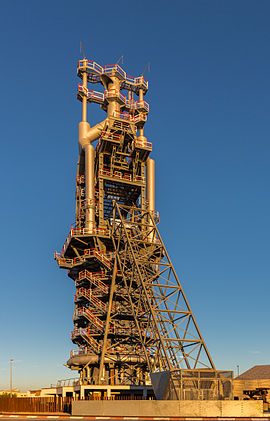
\includegraphics[width=3cm]{altoHorno.jpg}
    \caption{Podemos insertar imágenes.}
  \end{figure}

  Un alto horno es un cilindro con paredes de un cierto ancho. Dentro del mismo, se realiza la fusión de metales a temperaturas muy elevadas. Resulta útil calcular la isoterma de algún valor critico dentro de la pared, para prevenir que su estructura externa colapse.

  El objetivo del siguiente trabajo es, dadas las temperaturas internas y externas de las paredes de un alto horno y un valor, estimar la isoterma de ese valor.

  Al calcular la isoterma, se va a considerar un corte transversal de dicho horno. Para trabajar este problema computacionalmente, se discretizará el dominio en coordenadas polares.

  Se utilizará la ecuación de Laplace que permite relacionar cada punto del dominio con sus 4 vecinos. Esto genera un sistema de ecuaciones lineales que será resuelto utilizando los métodos numéricos de eliminación gaussiana y factorización LU.

  La eliminación gaussiana consiste en convertir la matriz del sistema en una matriz triangular superior y de esta forma simplificar el cálculo de las incógnitas utilizando sustitución hacia atrás.

  La factorización LU es un método similar al anterior pero no modifica el vector resultado y guarda los cambios que se le realizan a la matriz generada por el sistema al triangularla. Esto hace que para un mismo sistema de ecuaciones lineales con distintos resultados no sea necesario recalcular para cada uno la matriz triangulada, si  no que se realiza solo una vez y luego se afecta al vector resultado con los cambios guardados.

  % Ecuación de Laplace
  % Buscar citas en libros sobre eliminación gaussiana y factorización LU

\section{Desarrollo}

  Deben explicarse los métodos numéricos que utilizaron y su aplicación al problema concreto involucrado en el trabajo práctico. Se deben mencionar los pasos que siguieron para implementar los algoritmos, las dificultades que fueron encontrando y la descripción de cómo las fueron resolviendo. Explicar también cómo fueron planteadas y realizadas las mediciones experimentales.\footnote{Podemos hacer notas al pie.} Los ensayos fallidos, hipótesis y conjeturas equivocadas, experimentos y métodos malogrados deben figurar en esta sección, con una breve explicación de los motivos de estas fallas (en caso de ser conocidas).

  \[ \frac{\partial^2 T(r, \theta)}{\partial r^2} + \frac{1}{r} \frac{\partial T(r, \theta)}{\partial r} + \frac{1}{r^2} \frac{\partial^2 T(r, \theta)}{\partial \theta^2} = 0 \]

  Dados los parámetros de entrada, creamos una matriz asociada al sistema relacionando cada uno de los puntos del dominio con sus vecinos a través de la ecuación de Laplace.

  Así formamos una matriz diagonal dominante, lo que nos permite asegurarnos que el método de eliminación gaussiana se va a poder llevar a cabo sin necesidad de intercambiar filas, es decir, sin pivoteo.

\section{Resultados}

  Deben incluir los resultados de los experimentos, utilizando el formato más adecuado para su presentación. Deberán especificar claramente a qué experiencia corresponde cada resultado. No se incluirán aquí corridas de máquina.

\section{Discusión}

  Se incluirá aquí un análisis de los resultados obtenidos en la sección anterior (se analizará su validez, coherencia, etc.). Deben analizarse como mínimo los ítems pedidos en el enunciado. No es aceptable decir que ``los resultados fueron los esperados'', sin hacer clara referencia a la teoría a la cual se ajustan. Además, se deben mencionar los resultados interesantes y los casos ``patológicos'' encontrados.

\section{Conclusiones}

  Esta sección debe contener las conclusiones generales del trabajo. Se deben mencionar las relaciones de la discusión sobre las que se tiene certeza, junto con comentarios y observaciones generales aplicables a todo el proceso. Mencionar también posibles extensiones a los métodos, experimentos que hayan quedado pendientes, etc.

  \begin{enumerate}
    \item Podemos hacer listas numeradas
    \item ¡Con más de un item!
  \end{enumerate}

  \begin{itemize}
    \item Incluso podemos hacer
    \item listas con viñetas
    \item ¡que incluyan referencias a la bibliografía! ¡Sí! \cite{nosPodemosCopiarSiLoCitamos}
  \end{itemize}

\section{Apéndices}
\begin{subappendices}

  \subsection{Enunciado del trabajo práctico}

    En el apéndice A se incluirá el enunciado del TP.

  \subsection{Código fuente}

    En el apéndice B se incluirán los códigos fuente de las funciones relevantes desde el punto de vista numérico.

    \begin{algorithm}
      \caption{Podemos escribir pseudocódigo}
      \While{true}{
        $a \gets b$ \;
      }
    \end{algorithm}

    También podemos incluir archivos de código:
    \lstinputlisting[language=C++, firstline=0, lastline=18, style=customcpp]{../src/altohorno.cpp}

  \subsection{Otras cosillas}

    Resultados que valga la pena mencionar en el trabajo pero que sean demasiado específicos para aparecer en el cuerpo principal del trabajo podrán mencionarse en sucesivos apéndices rotulados con las letras mayusculas del alfabeto romano. Por ejemplo: la demostración de una propiedad que aplican para optimizar el algoritmo que programaron para resolver un problema.

\end{subappendices}

\begin{thebibliography}{1}

  \bibitem{referencias} Es importante incluir referencias a libros, artículos y páginas de Internet consultados durante el desarrollo del trabajo, haciendo referencia a estos materiales a lo largo del informe.
  \bibitem{nosPodemosCopiarSiLoCitamos} Se deben citar también las comunicaciones personales con otros grupos.

\end{thebibliography}

\end{document}
